\begin{figure}[ht]
\centering
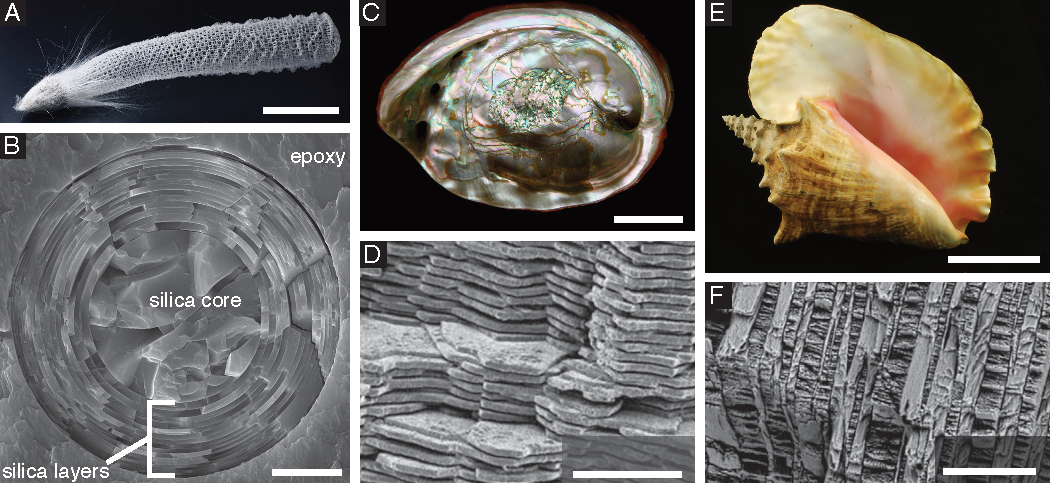
\includegraphics[width=\textwidth]{Figures/Figure1_V4.pdf}
\caption{Examples of layered architectures in biological materials. (\textsf{A}) The shell of \textit{Haliotis rufescens}---the red abalone (image courtesy of John Varner). (\textsf{B}) A scanning electron microscope (SEM) image of nacre from \textit{H. rufescens} showing its brick and mortar layered architecture (modified with permission from~\cite{rabiei2012nacre} copyright 2012, the Royal Society of Chemistry). (\textsf{C}) The shell of \textit{Strombus gigas}---the queen conch (image courtesy of John Varner). (\textsf{D}) the layered architecture of the \textit{S. gigas} shell (modified with permission from ~\cite{osuna2014shell} copyright 2014, Elsevier). (\textsf{E}) A force-displacement curve from a three-point bending test performed on a synthetic laminated material (adapted from~\cite{clegg1990simple}). (\textsf{F}) An image of a lamellar composite material consisting of silicon carbide sheets with graphite interface tested in three-point bending (modified from~\cite{clegg1990simple}).}
\label{fig:arch}
\end{figure}
